\begin{table*}
\vspace{-10pt}
\centering
\begin{tabular}{lcccccccc}
\toprule
\multirow{2}{*}{Model} & \multirow{2}{*}{SEP-28K Test}  & \multicolumn{6}{c}{SEP-28K - Fluency Bank} \\
\cmidrule{3-8}
 &   & All	& Blocks & Interjections & Prolongation & Sound Rep. & Word Rep.\\
% &   & All & Bl & Int & Pro & Snd & Wd \\
\midrule
Baseline~\cite{bayerl22b_interspeech}$^\dagger$ & -- &
 --   & 0.33 &	\textbf{0.84} &	0.60 &	0.60 &	0.43 \\
Baseline~\cite{bayerl23_interspeech}$^\dagger$ & -- &
 --     & 0.17 & \underline{0.82} & 0.60 & 0.63 & 0.47 \\
\midrule
Baseline~\cite{harvill22_interspeech} & 0.700 &
0.68 &	0.34 &	0.62 &	0.28 &	0.39 &	0.39 \\

% \midrule
% WavLMLg + HConv. & \textbf{0.785} &
% \textbf{0.82} &	\textbf{0.61} &	0.61 &	\textbf{0.60} &	\textbf{0.72} &	\textbf{0.65} \\
WavLMLg + HConv. & \underline{0.800} &	\textbf{0.85} &	\textbf{0.63} &	0.59 &	\textbf{0.63} &	\textbf{0.75} &	\textbf{0.70} \\
WavLMLg + HConv. + CTC & \textbf{0.803} &	\underline{0.84} &	\underline{0.62} &	0.57 &	\underline{0.61} &	\underline{0.74} &	\underline{0.67} \\


\midrule
 & \multicolumn{7}{c}{\textit{Using Weighted Sum~(WS)}} \\
 \cmidrule(lr){2-8}
WavLMLg + WS & 0.789 &	0.82 &	0.58 &	0.63 &	0.54 &	0.70 &	0.63 \\
WavLMLg + WS + CTC & 0.790 &	0.82 &	0.59 &	0.59 &	0.55 &	0.69 &	0.62 \\
% \midrule
% WavLMBs + HConv. & 0.670 &	0.68 &	0.33 &	0.59 &	0.31 &	0.43 &	0.35 \\
% WavLMBs + HConv. + CTC & 0.674 &	0.69 &	0.35 &	0.62 &	0.30 &	0.45 &	0.36 \\

\midrule
 & \multicolumn{7}{c}{\textit{Different Finetune Dataset Size using ``WavLMLg + HConv. + CTC''}} \\
\cmidrule(lr){2-8}
Data Ratio: $0\%$ &
0.685 &	0.70 &	0.36 &	0.59 &	0.31 &	0.43 &	0.37 \\
Data Ratio: $25\%$ &
0.774 &	0.82 &	0.62 &	0.58 &	0.61 &	0.77 &	0.72 \\
Data Ratio: $50\%$ &
0.798 &	0.84 &	0.65 &	0.57 &	0.64 &	0.76 &	0.71 \\
Data Ratio: $75\%$ &
0.793 &	0.83 &	0.66 &	0.56 &	0.65 &	0.79 &	0.74 \\
Data Ratio: $100\%$ & 0.803 &	0.84 &	0.62 &	0.57 &	0.61 & 0.74 &	0.67 \\








% WavLM + HierConv. + VC & 0.783 &
% 0.80 &	0.54 &	0.60 &	0.50 &	0.66 &	0.59 \\
\bottomrule
\end{tabular}
\caption{Utterance Level Stuttered Speech Detection Evaluation on SEP-28K and Fluency Bank. The numbers are F1 scores.
Notice that for models with $^\dagger$, they are trained to distinguish different stuttering types while training. Also the numbers are directly reported from their paper.}
\label{tab:Utt_level}
\vspace{-5pt}
\end{table*}

While we aim to evaluate the performance of our model on word-level stuttered speech detection,  we also want to compare it with previous works that studied utterance-level stuttering detection.
Hence, we evaluate under both the utterance-level and word-level stuttering detection conditions.
For the former, we evaluate on SEP-28K testing set and also report the F1 score for each stuttering type on Fluency Bank (a subset of SEP-28K).
For the latter, we evaluate models on our word-level stuttering dataset and report F1, precision, and recall on each partition separately.
Additionally, we report the F1 score and Average precision on the entire dataset.
We choose to report F1 score instead of other metrics such as accuracy due to the fact that the data is highly imbalanced~(There are many more non-stuttered speech segments than stuttered segments).
We sweep the detection threshold from 0 to 1 with a step of 0.05 to find the optimal threshold for all settings.
Throughout our evaluation, we found out that the word-level dataset is very sensitive to the threshold selection.
Hence, we also report Average Precision on the entire word-level stuttered speech dataset.
F1 score on the one hand is more intuitive but sensitive to threshold selection especially on this dataset, while Average Precision is a threshold-independent metric that evaluates the classification model under all possible thresholds.
With these two evaluation benchmarks, we further conduct ablation experiments on the effect of CTC loss, the SSL interface/model selection, and the size of the finetuning dataset.
Finally, we show some qualitative examples of our model's outputs.

\vspace{-10pt}
\subsection{Utterance Level stuttered speech detection}
Since our model is only trained to detect stuttering events and not to distinguish between different types of stuttering, we report the type-specific stuttering detection F1 score by selecting different subsets of the testing dataset.
For example, to test the F1 score for blocks on SEP-28K - Fluency Bank, we filter the testing set to include only utterances with blocks and utterances without stuttering.

As shown in Table~\ref{tab:Utt_level}, overall, our model surpasses the baseline systems.
Specifically, \cite{bayerl22b_interspeech,bayerl23_interspeech} and our model outperforms ~\cite{harvill22_interspeech} by a large margin, indicating the benefit of using Speech SSL models and probably the transformer architecture.
Interestingly, our model beats \cite{bayerl22b_interspeech,bayerl23_interspeech} in general, except for interjections.
This could potentially be improved by adding synthesized sound interjections in the pretraining stage.

\vspace{-10pt}
\subsection{Word Level stuttered speech detection}
\begin{table*}
\centering
\begin{tabular}{lccccccccccc}
\toprule
\multirow{2}{*}{Model} & \multicolumn{2}{c}{All} &  \multicolumn{3}{c}{Stut. Blngl. Speech} & \multicolumn{3}{c}{Non-stut. Blngl. Speech} &  \multicolumn{3}{c}{Stut. Fluency Bank} \\
\cmidrule(lr){2-3}
\cmidrule(lr){4-6}
\cmidrule(lr){7-9}
\cmidrule(lr){10-12}
   & F1 & Avg.~P & 
 F1	& P & R & 
 F1	& P & R & 
 F1	& P & R \\
\midrule
Baseline~\cite{harvill22_interspeech}& 0.411 & 0.864 &
0.389 &	0.360 &	0.423 &	
0.342 &	0.245 &	0.565 &	
0.440 &	0.315 &	0.728 \\

WavLMLg + HConv. & 
	0.536 & 0.899  &	0.484 &	0.364 &	0.723 &	0.496 &	0.391 &	0.680 &	0.585 &	0.496 &	0.715 \\

WavLMLg + HConv.+ CTC &
	\textbf{0.554} & \textbf{0.927}  &	\textbf{0.490} &	0.375 &	0.708 &	\textbf{0.518} &	0.439 &	0.633 &	0.591 &	0.508 &	0.708 \\

\midrule
 & \multicolumn{10}{c}{\textit{Using Weighted Sum~(WS)}} \\
\cmidrule(lr){2-12}
WavLMLg + WS. &
	0.536 & 0.898 &	0.425 &	0.356 &	0.529 &	0.425 &	0.356 &	0.529 &	0.594 &	0.507 &	0.718 \\


WavLMLg + WS. + CTC &
	0.540 & 0.888 &	0.460 &	0.336 &	0.730 &	0.403 &	0.344 &	0.486 &	\textbf{0.603} &	0.514 &	0.729 \\
% \midrule
%  & \multicolumn{10}{c}{\textit{Using WavLM Base}} \\
% \cmidrule(lr){2-11}

% WavLMBs + HConv. & 0.361 & 0.334 &	0.200 &	1.000 &			0.273 &	0.158 &	1.000 &	0.406 &	0.304 &	0.610 \\
% WavLMBs + HConv. + CTC & 0.354  & 0.349 &	0.243 &	0.620 &			0.273 &	0.158 &	1.000 &	0.395 &	0.246 &	1.000 \\

\midrule
 & \multicolumn{10}{c}{\textit{Select Single WavLM Large Layer}} \\
\cmidrule(lr){2-12}









WavLMLg Layer~0 & 0.439 & 0.864 &	0.340 &	0.214 &	0.825 &	0.279 &	0.192 &	0.507 & 0.519 & 0.415 & 0.694 \\
WavLMLg Layer~4 & 0.479 & 0.876 &	0.403 &	0.292 &	0.650 &	0.332 &	0.256 &	0.471 & 0.539 & 0.434 & 0.709 \\
WavLMLg Layer~8 & 0.499 & 0.875 &	0.442 &	0.389 &	0.511 &	0.424 &	0.341 &	0.561 & 0.541 & 0.476 & 0.628 \\
WavLMLg Layer~12 & 0.522 & 0.891 &	0.458 &	0.331 &	0.745 &	0.417 &	0.334 &	0.554 & 0.581 & 0.493 & 0.707 \\
WavLMLg Layer~16 & 0.548 & 0.910 &	0.480 &	0.418 &	0.562 &	0.513 &	0.462 &	0.576 & 0.589 & 0.513 & 0.692 \\
WavLMLg Layer~20 & 0.552 & 0.903 &	0.486 &	0.378 &	0.679 &	0.488 &	0.415 &	0.594 & 0.592 & 0.521 & 0.684 \\
% WavLMLg Layer~22 &0.561 & 0.907 &	0.500 &	0.384 &	0.715 &	0.470 &	0.406 &	0.558 &	0.610 &	0.533 &	0.712 \\
WavLMLg Layer~22 &	0.550 &  0.912 &	0.488 &	0.361 &	0.752 &	0.484 &	0.391 &	0.633 &	0.590 &	0.522 &	0.679 \\

WavLMLg Layer~24 & 0.504 & 0.901 &	0.464 &	0.366 &	0.635 &	0.429 &	0.345 &	0.568 & 0.546 & 0.470 & 0.651 \\

% Baseline~\cite{harvill22_interspeech} & 0.700 &
% 0.68 &	0.34 &	0.62 &	0.28 &	0.39 &	0.39 \\
% \midrule
% WavLM + HierConv. & 0.785 &
% 0.82 &	0.61 &	0.61 &	0.60 &	0.72 &	0.65 \\
% WavLM + HierConv. + VC & 0.783 &
% 0.80 &	0.54 &	0.60 &	0.50 &	0.66 &	0.59 \\



\midrule
 & \multicolumn{10}{c}{\textit{Different Finetune Dataset Size using ``WavLMLg + HConv. + CTC''}} \\
\cmidrule(lr){2-12}
Data Ratio: $0\%$  &
 0.469 & 0.872 & 0.377 & 0.299 & 0.511 & 0.305 & 0.259 & 0.371 & 0.545 & 0.457 & 0.674 \\
Data Ratio: $25\%$ &
  0.530 & 0.892 & 0.471 &  0.405 & 0.562 & 0.362 & 0.452 & 0.302 &	0.579 &	0.487 &	0.713 \\
Data Ratio: $50\%$ &
0.533 & 0.904 &	0.470 &	0.338 &	0.774 &	0.493 &	0.413 &	0.612 &	0.579 &	0.487 &	0.713 \\
Data Ratio: $75\%$ &
0.516 & 0.888 &	0.460 &	0.368 &	0.613 &	0.386 &	0.417 &	0.360 &	0.557 &	0.472 &	0.678 \\
Data Ratio: $100\%$ &
0.554 & 0.927  &	0.490 &	0.375 &	0.708 &	0.518 &	0.439 &	0.633 &	0.591 &	0.508 &	0.708 \\
%     WavLMLg + HConv. Ft$_{1}$ &
% f1 &
%  & & &
%  & & &
%  & & \\








% 0.516	0.460	0.368	0.613	0.386	0.417	0.360	0.557	0.472	0.678

\bottomrule
\end{tabular}
\caption{Word Level Stuttered Speech Detection Evaluation. ``WavLMLg'' stands for WavLM Large.
HConv. indicates Hierarchical Convolution Interface and WS means weighted sum interface. For the metrics, ``Avg.~P'' stands for Average Precision while ``P'' and ``R'' indicate precision and recall respectively.
``Stut. Blngl. Speech'' and ``Non-stut. Blngl. Speech'' stands for Stuttering Bilinguals Speech and Non-stuttering Bilinguals Speech.
}
\label{tab:Word_level}
\vspace{-10pt}
\end{table*}

In Table~\ref{tab:Word_level}, overall ``WavLMLg + HConv. + CTC'' outperforms the baseline model and other variations.
In terms of different partitions, Fluency Bank has the highest F1 scores regardless of method.
The reason might be the difference between native speakers and bilingual speakers.
For Bilinguals Speech, stuttering bilinguals tend to have higher F1 scores compared to non-stuttering bilinguals.
The reason is that our model tends to have a high recall and a low precision in most cases, which is also true for the baseline model.
Compared to the baseline method, our model improves more on recall than precision.
One avenue for future work would be to incorporate an improved prior over where stuttered speech is likely to occur within an utterance or a better way to condition the model on different patient demographics.

\vspace{-10pt}
\subsection{The effect of CTC loss and SSL interface selection}
To study the effect of CTC loss and HConv. Interface we design several ablation experiments.
For the utilization of WavLM, we design models using weighted sum~(which is a set of learnable weights that is multiplied layer-wisely on WavLM Large hidden layers and sum up) or simply select a single layer.
Due to the extensive computing, we select every 4 layers of WavLM Large for our experiment.
For HConv. and Weighted Sum, we also try adding CTC loss or not.

\begin{figure}
\centering
% 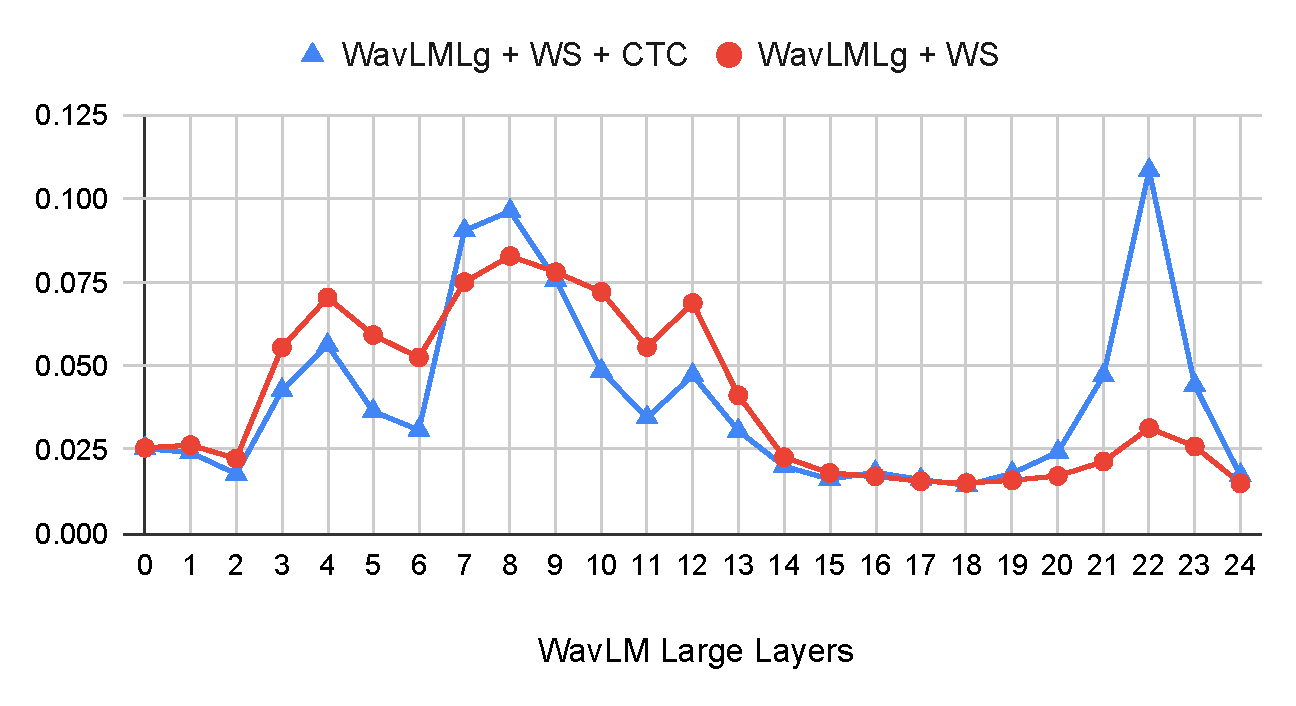
\includegraphics[width=0.5\textwidth,trim={0.2cm 0.6cm 0cm 0.4cm},clip]{figs/pdfs/ws_dist.pdf}
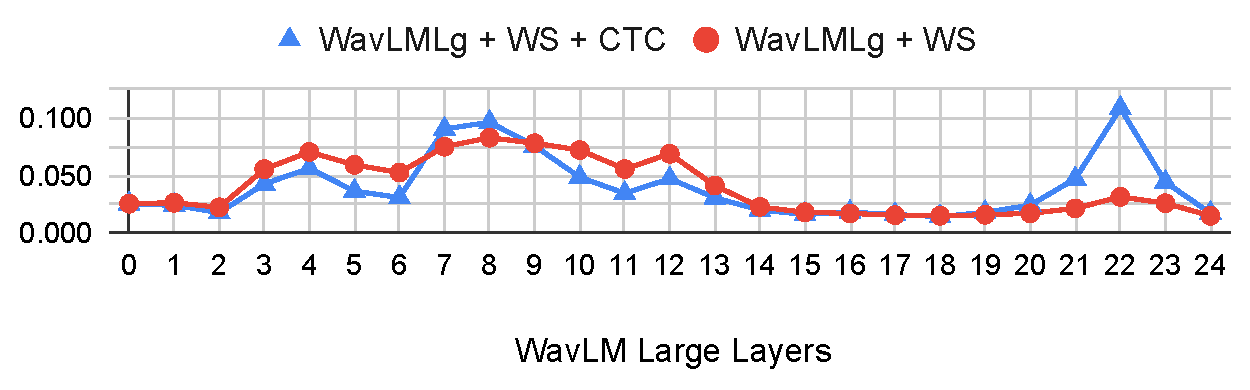
\includegraphics[width=0.5\textwidth,trim={0.3cm 0.3cm 0.3cm 0.4cm},clip]{figs/pdfs/ws_dist_small.pdf}
\caption{The learned weights distribution of weighted sum interface in WavLMLg + WS and WavLMLg + WS + CTC.}
\label{fig:ws_dist}
\vspace{-10pt}
\end{figure}
\begin{figure*}[h]
\centering
% 6 examples
% 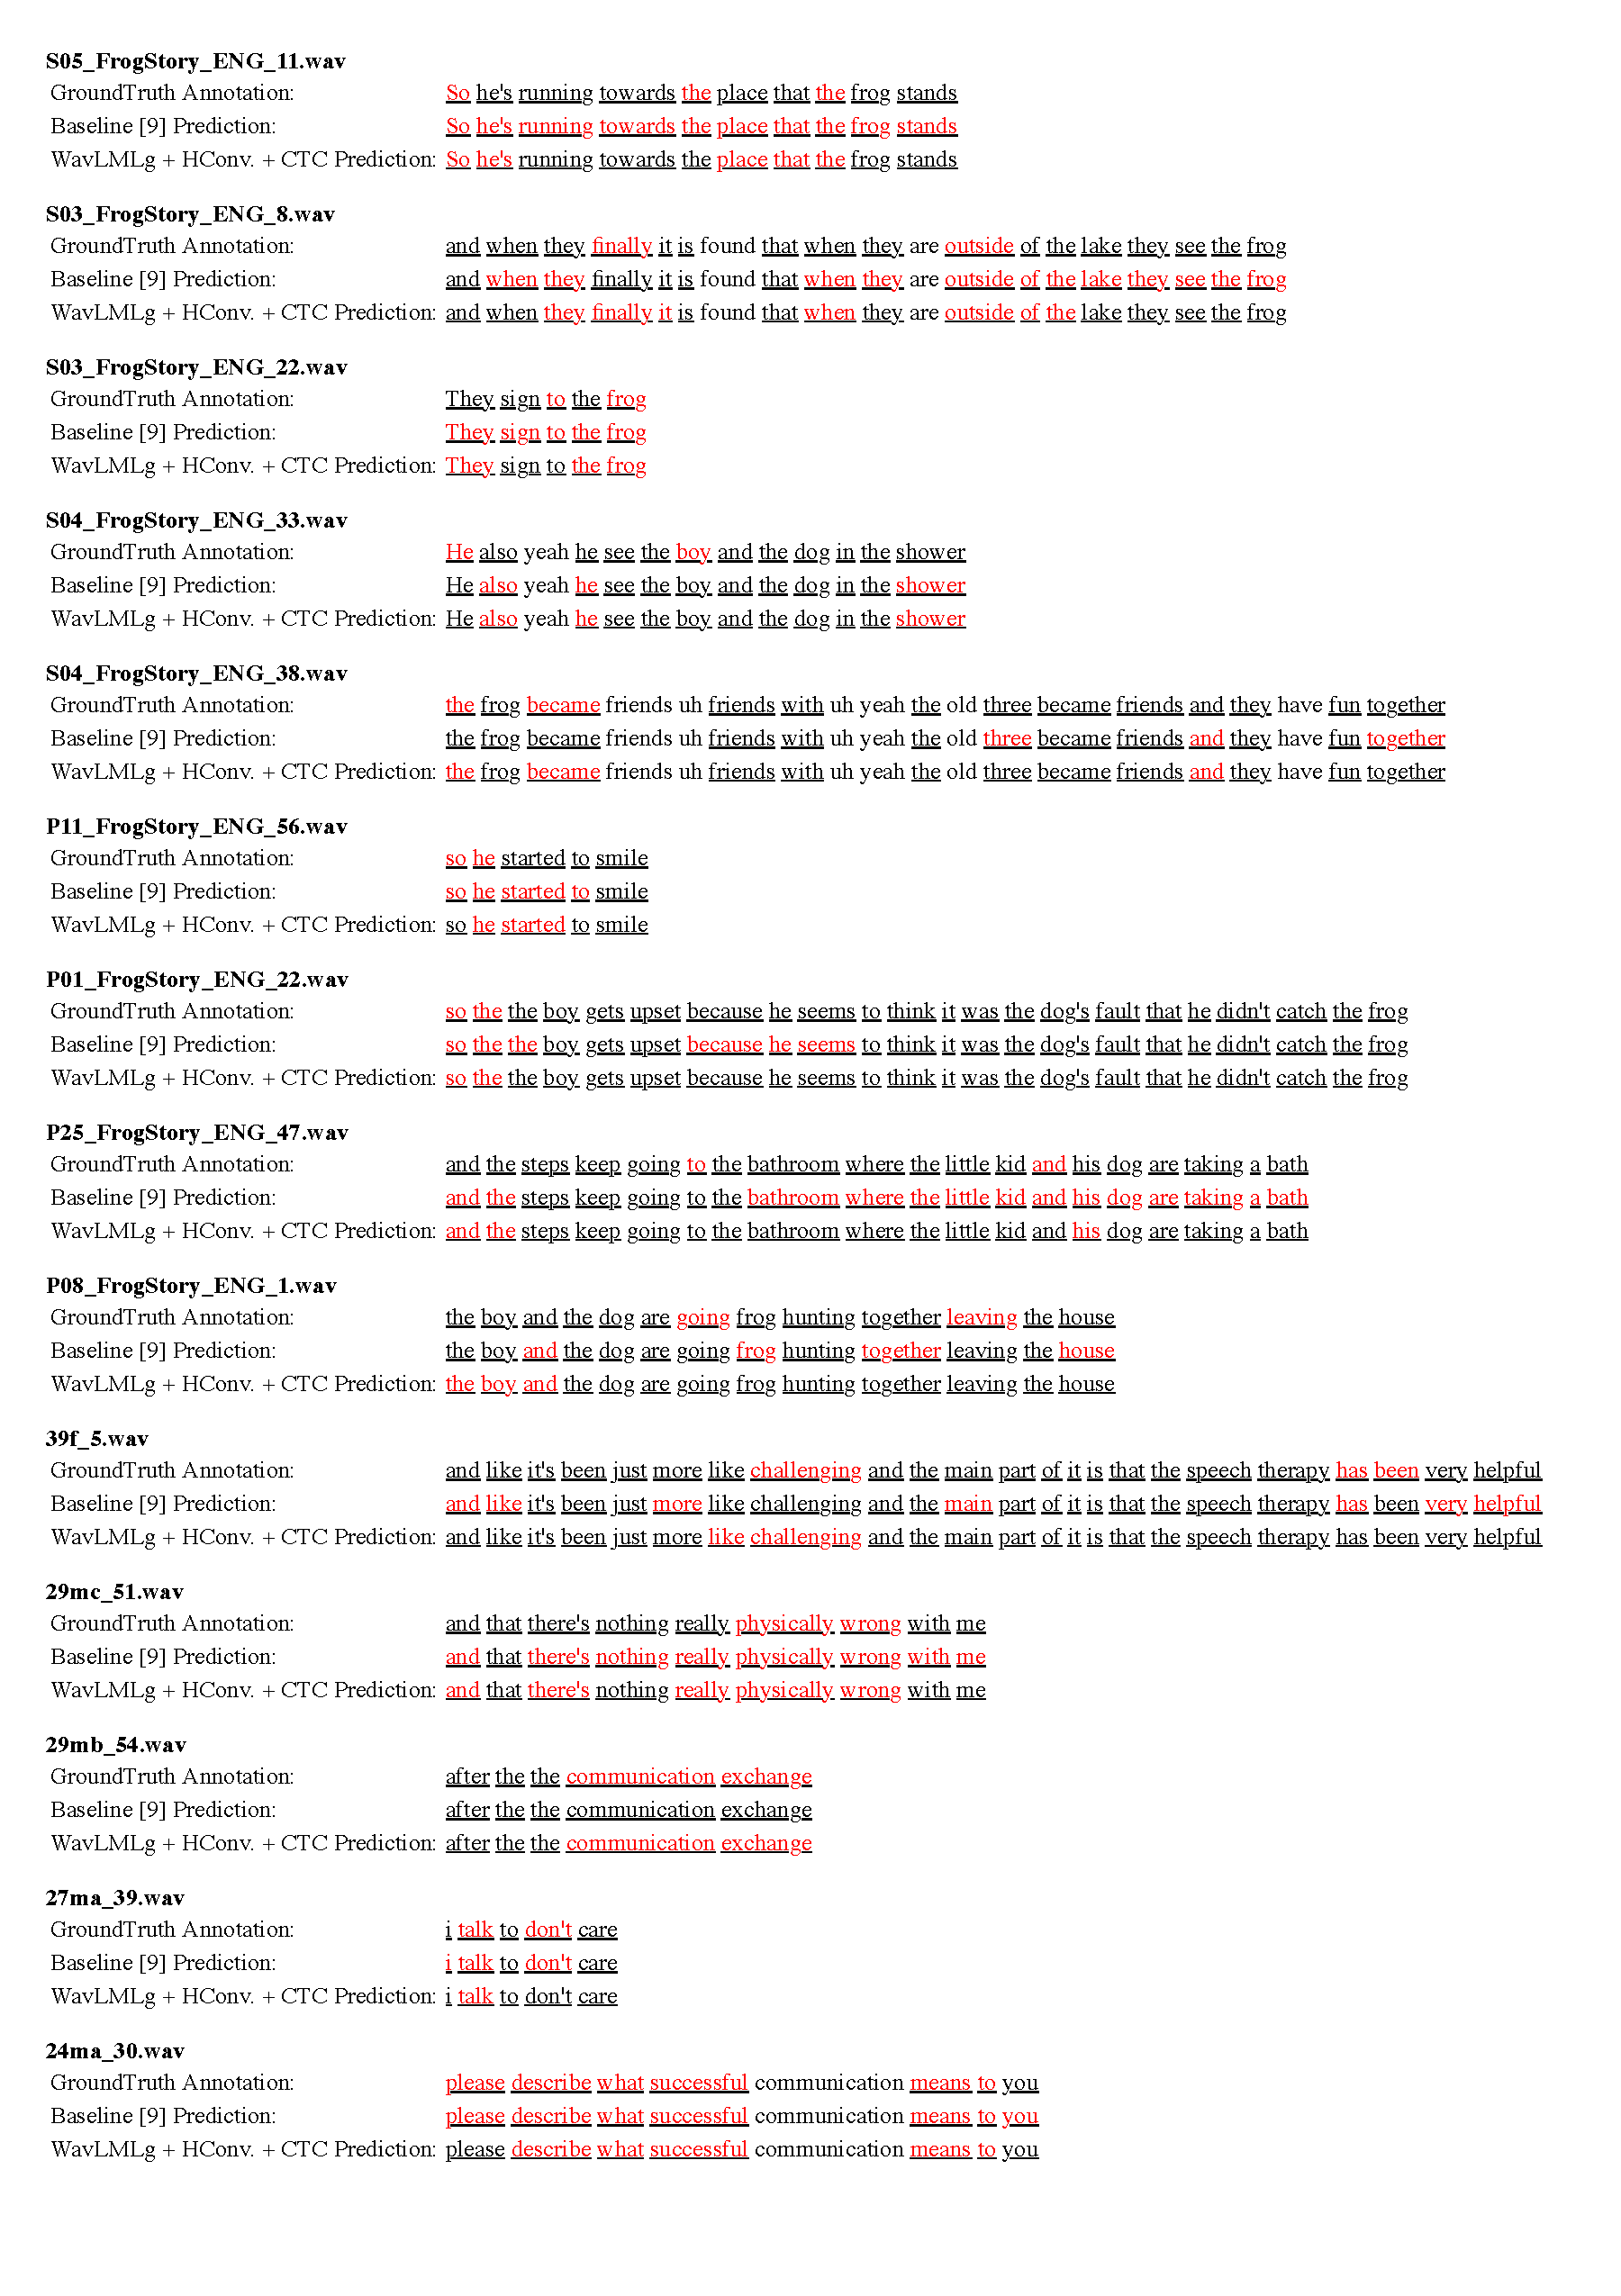
\includegraphics[width=0.9\textwidth,trim={0.2cm 26cm 6cm 0.9cm},clip]{figs/pdfs/qualitative_examples.pdf}
% 3 examples
% 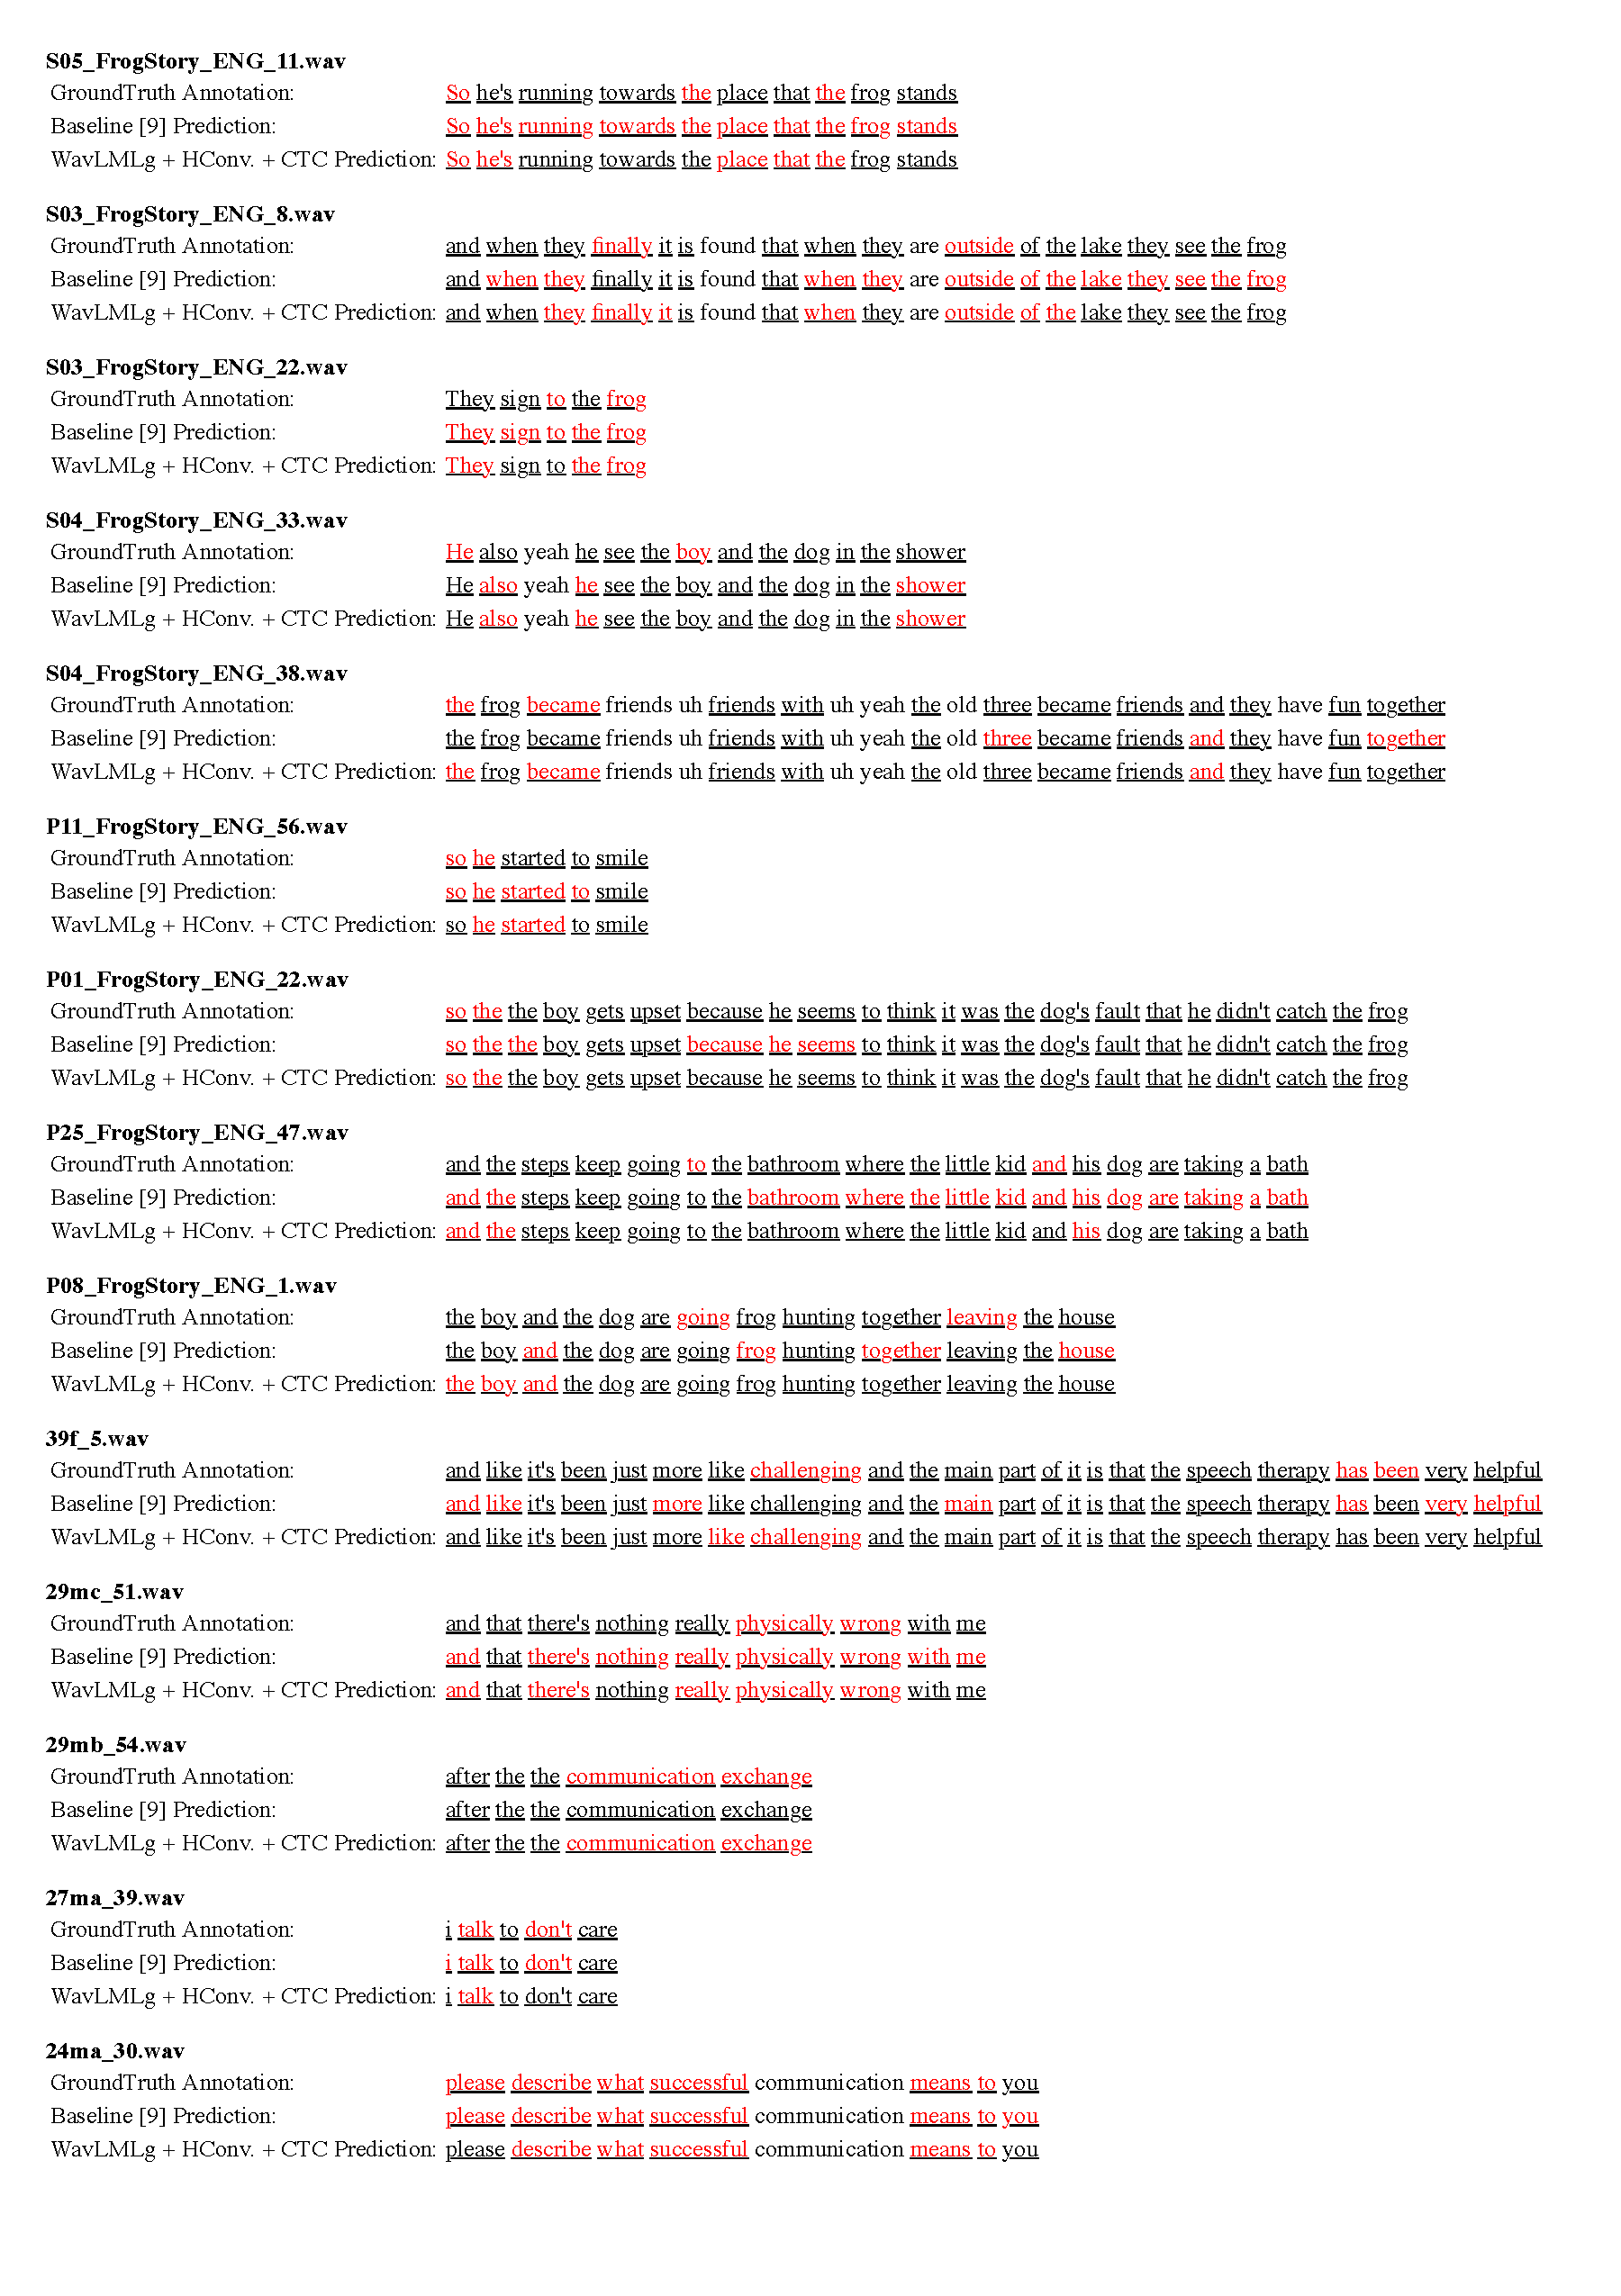
\includegraphics[width=0.9\textwidth,trim={0.2cm 34cm 6cm 0.9cm},clip]{figs/pdfs/qualitative_examples.pdf}
% 2 examples (title)
% 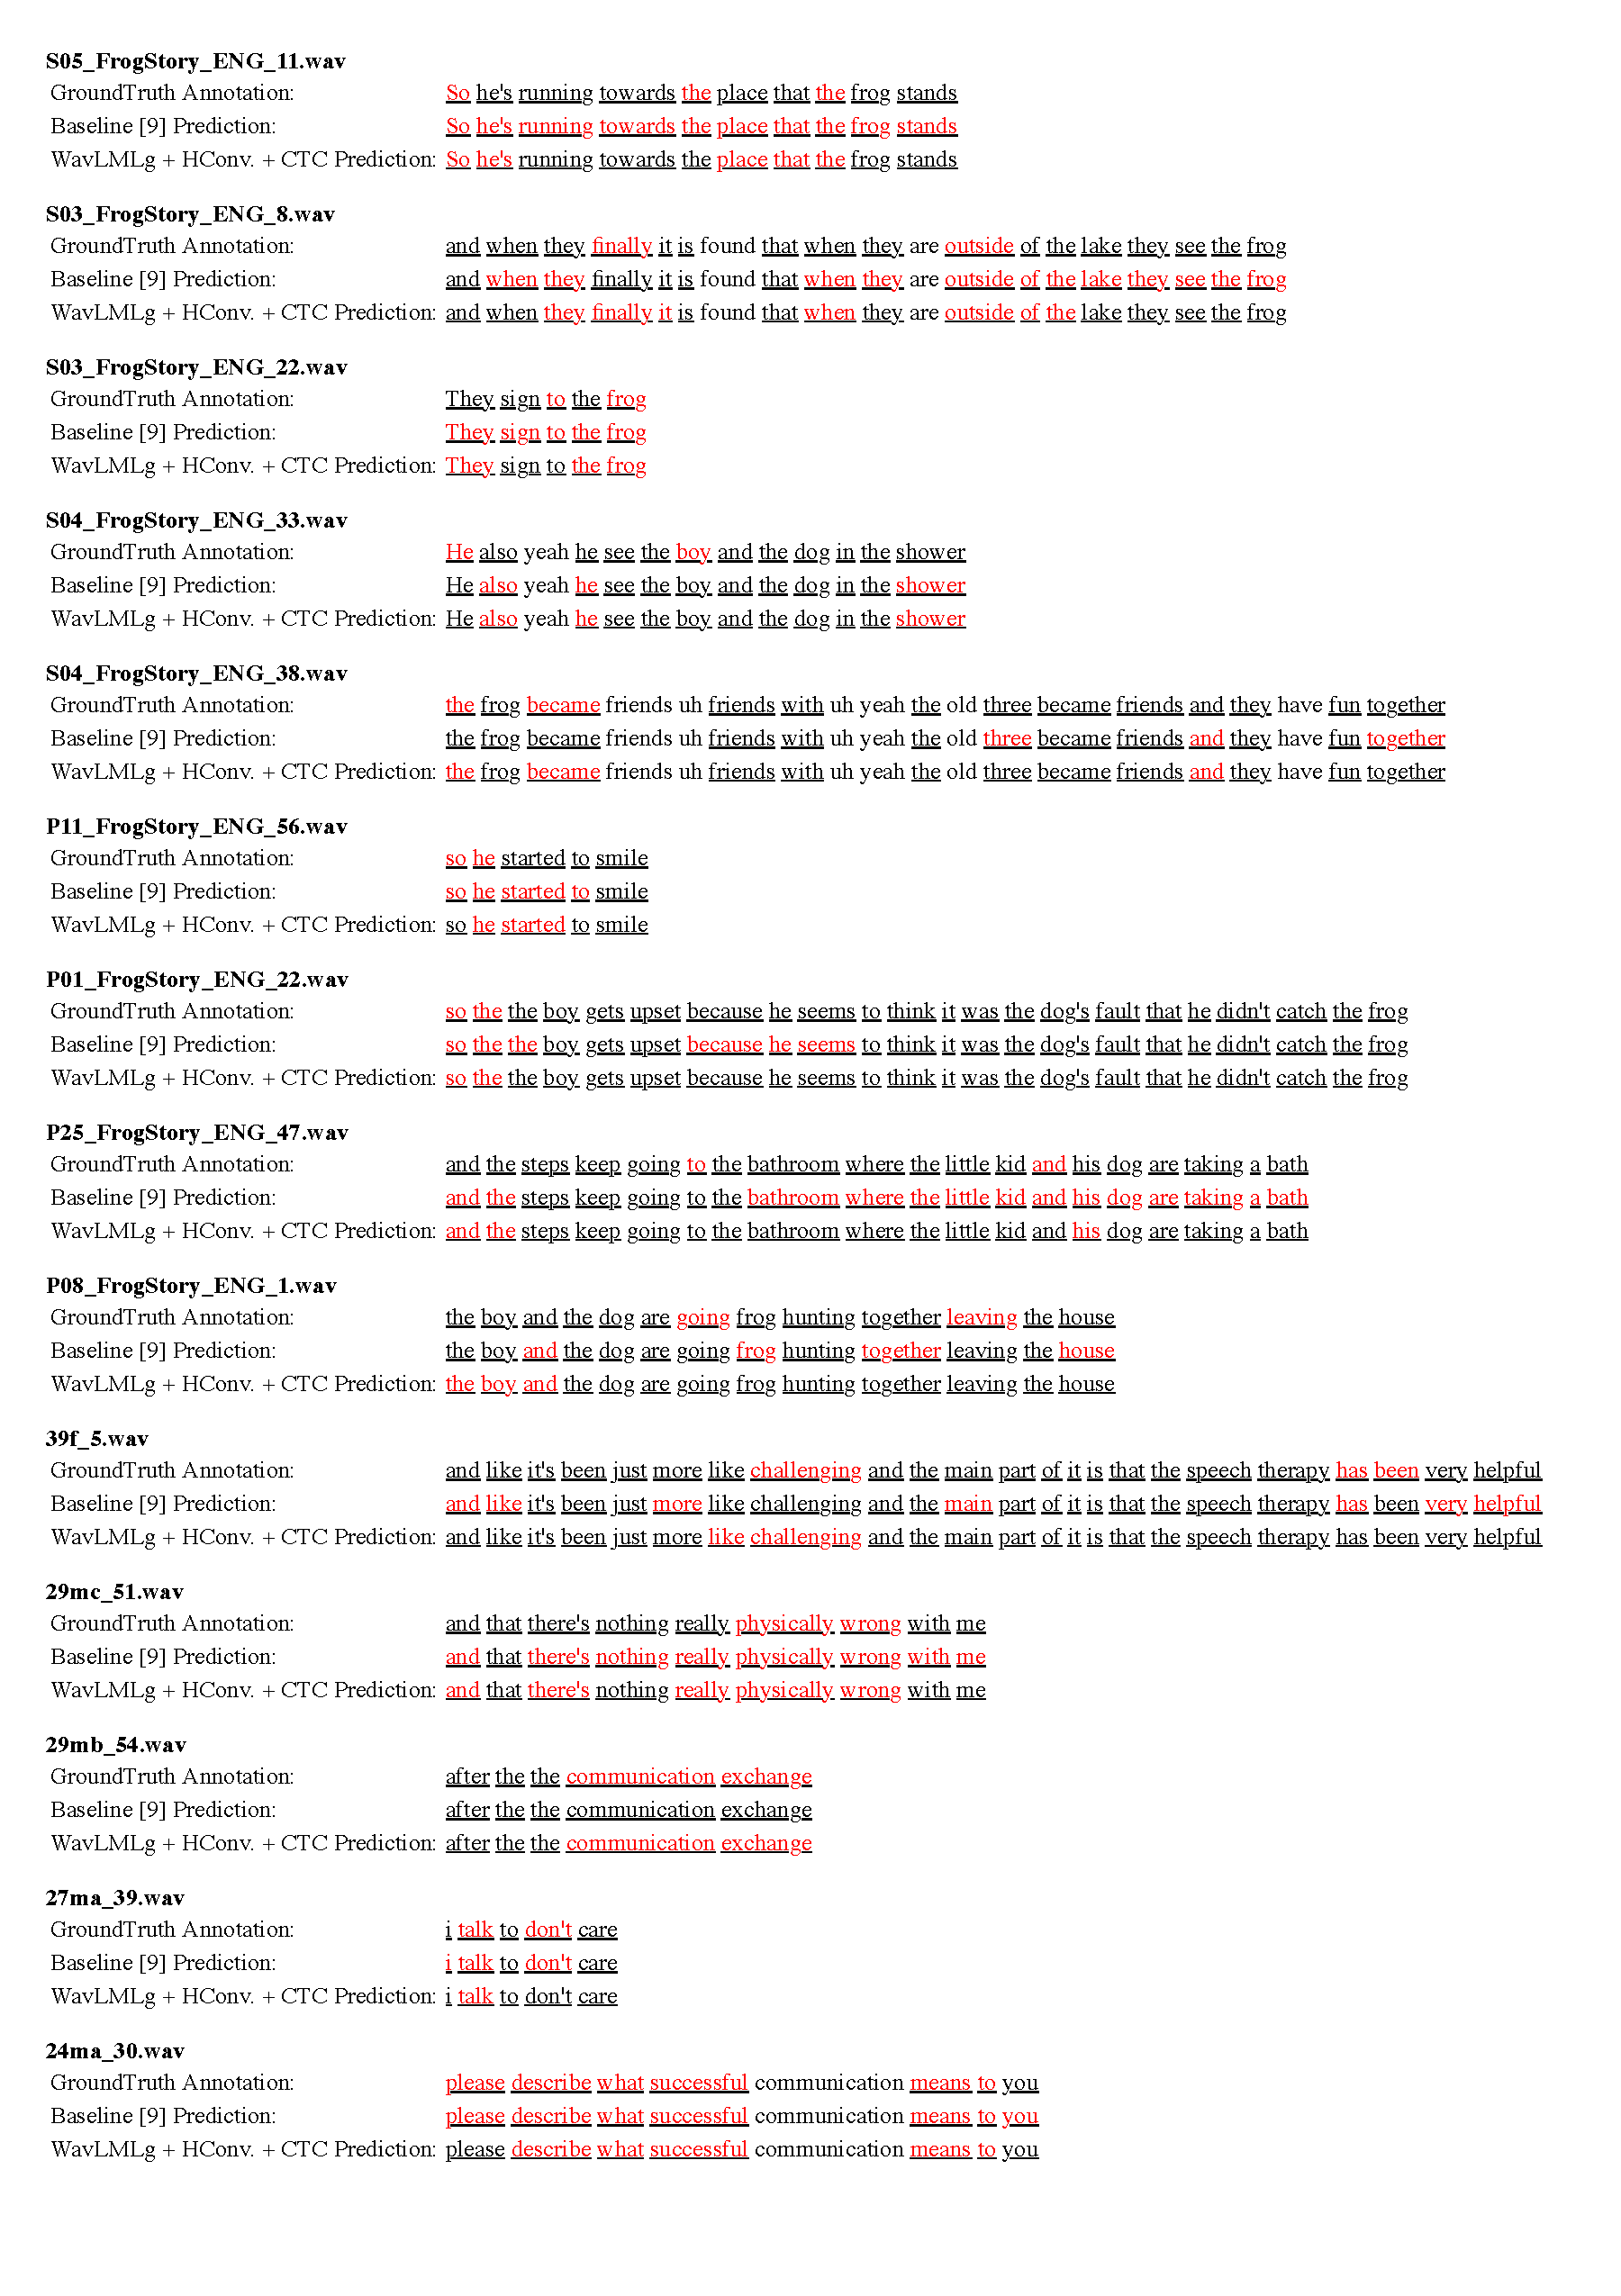
\includegraphics[width=0.9\textwidth,trim={0.2cm 37cm 6cm 0.9cm},clip]{figs/pdfs/qualitative_examples.pdf}
% 2 examples (no title)
% 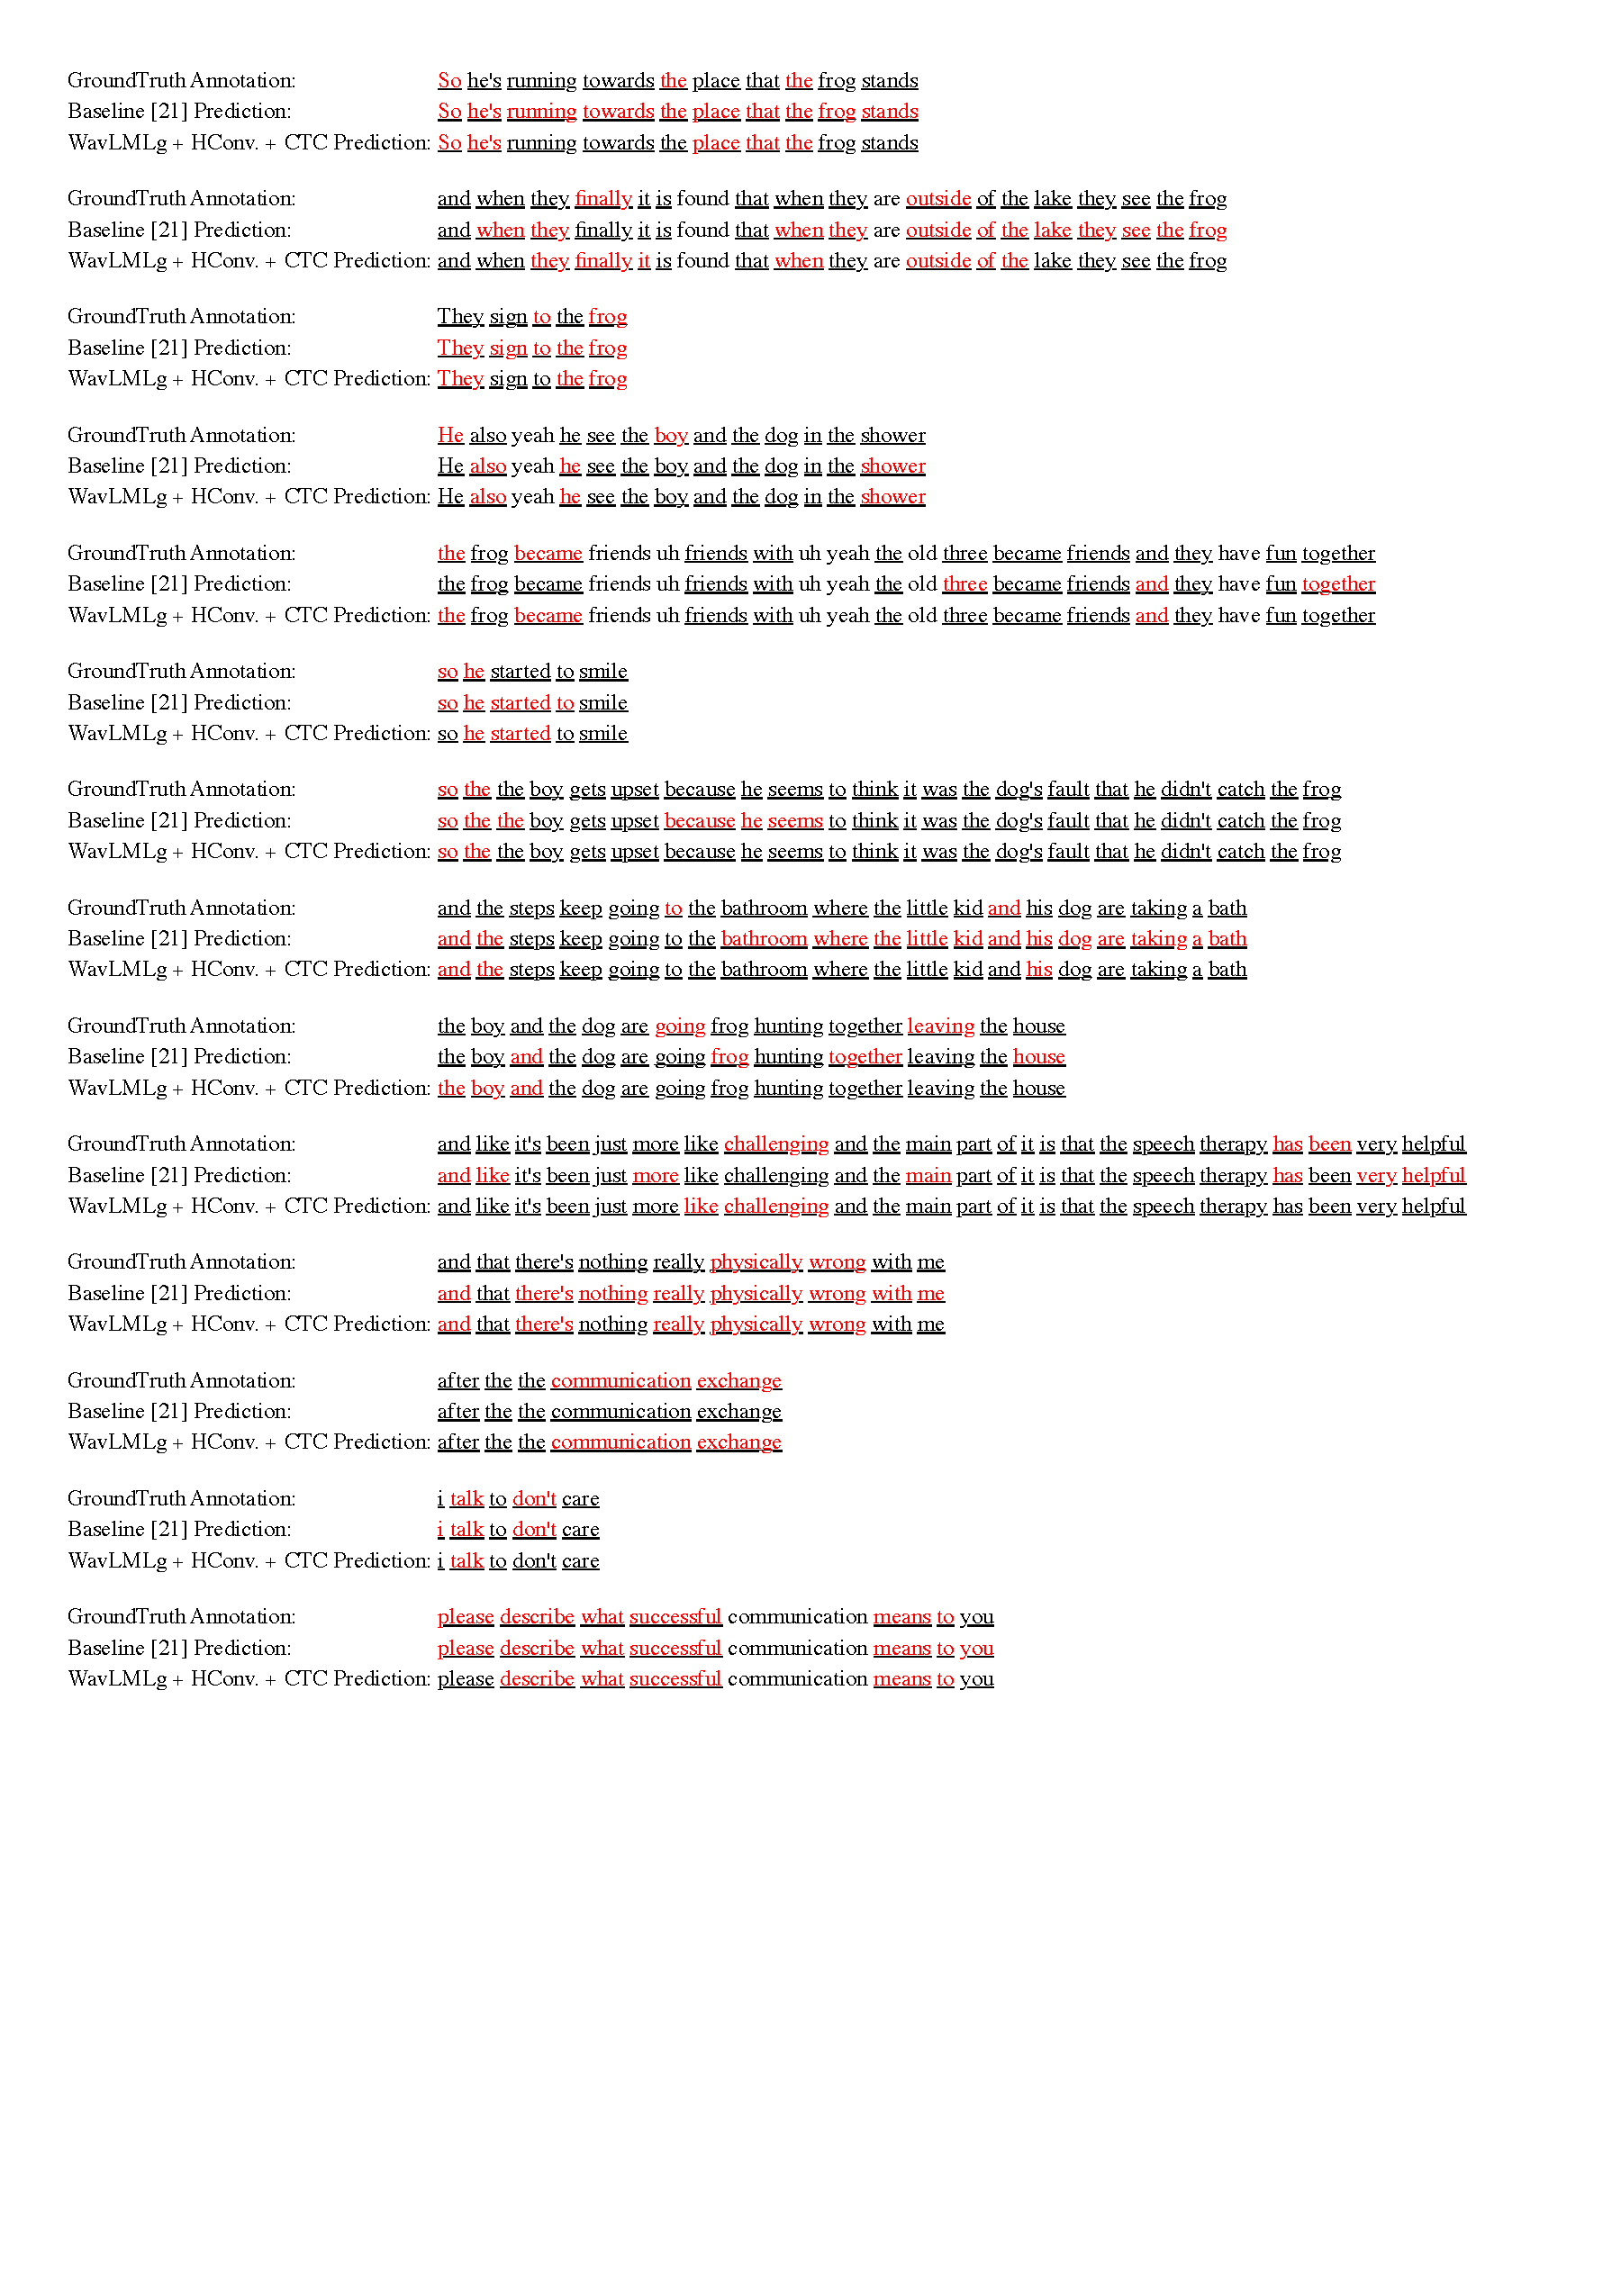
\includegraphics[width=0.9\textwidth,trim={0.2cm 38cm 7.4cm 0.9cm},clip]{figs/pdfs/qualitative_examples_noTitle.pdf}
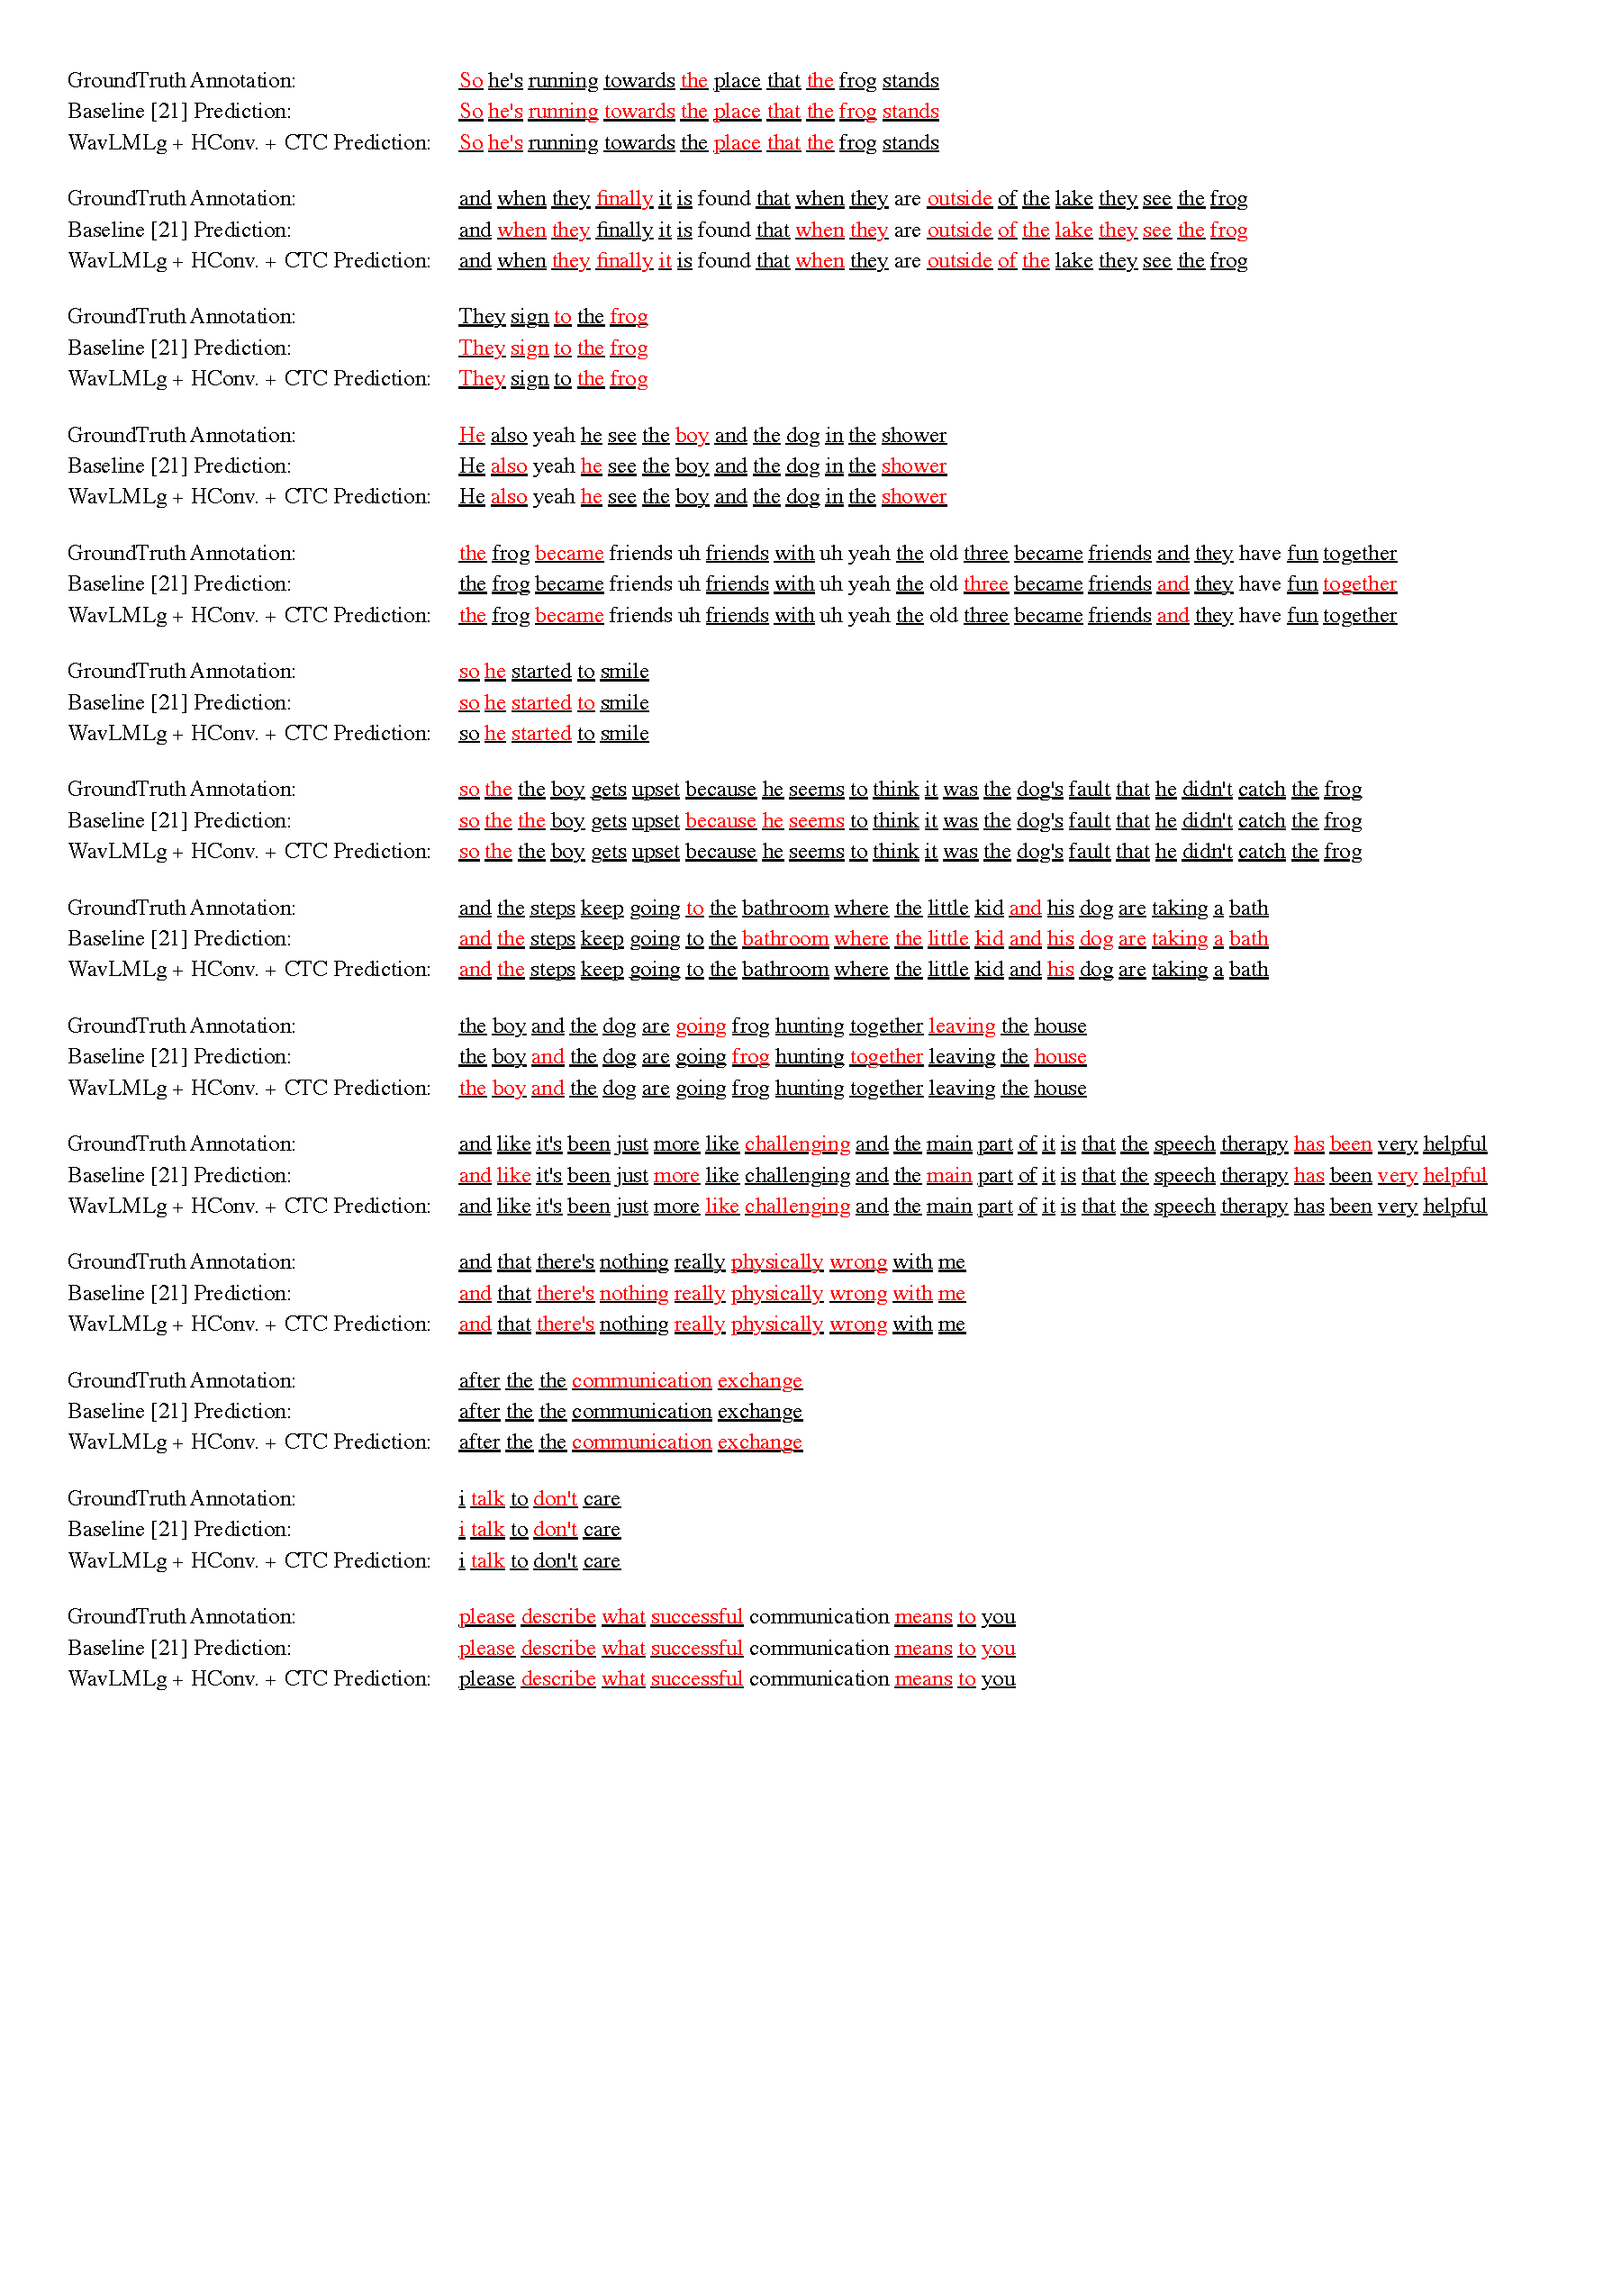
\includegraphics[width=0.9\textwidth,trim={0.2cm 38cm 7cm 0.9cm},clip]{figs/pdfs/qualitative_examples_noTitle_pad16.pdf}
\caption{Examples of our model and baseline model on word-level stuttering speech detection. Only the words with underscores are considered when evaluating. Words in red indicate that it is categorized as stuttered speech.
% \ian{will update the citation index for baseline later.} \david{maybe trim the number of examples here}
}
\label{fig:qualititave_examples}
\vspace{-10pt}
\end{figure*}
On the utterance level (See Table~\ref{tab:Word_level}), we see that with the help of CTC loss, the performance with both HConv. and  Weighted Sum layer aggregation strategies improved.
Interestingly, without CTC loss, both interfaces perform roughly the same overall.
We hypothesize that HConv. could benefit more from the guidance of CTC loss in terms of word-level stuttered speech detection.
The same trend can also be observed on the word-level stuttering speech dataset in Table~\ref{tab:Word_level}.
Hence, we further visualize the learned weights of the weighted sum in ``WavLMLg + WS'' and ``WavLMLg + WS + CTC'' in Figure~\ref{fig:ws_dist}.
With the help of CTC loss, the weight distribution becomes more concentrated on the peaks, indicating that CTC loss is helping the model to learn a better way of utilizing upstream model features.

We also report the performance of using a single layer from WavLM-Large in Table~\ref{tab:Word_level}.
Besides experiments with every four layers of WavLM-Large, we also include an experiment using the 22nd layer of WavLM-Large according to the layer with the highest learned weight in Figure~\ref{fig:ws_dist}.
Interestingly, layers 8 and 22 have the highest learned weights, but overall the best performance falls roughly on the upper half of WavLM-Large layers~(from layer 12 to 24).
We note that ``WavLMLg Layer 22'' has an overall F1 score close to our best model ``WavLMLg + HConv.+ CTC'', but falls behind in terms of average precision, indicating that the HConv. interface is an effective approach to utilizing WavLM-Large on word-level stuttered speech detection.

\vspace{-14pt}
\subsection{The effect of different Speech SSL models}
\begin{table}
\centering
\small
\begin{tabular}{lcc}
\toprule
% \multirow{2}{*}{Model} & All &  \multicolumn{3}{c}{Stut. FrgStry} & \multicolumn{3}{c}{Non Stut. FrgStry} &  \multicolumn{3}{c}{Stut. Fluency Bank} \\
Model & SEP-28K Test & Word Level Stuttered 
\\
\midrule
% \cmidrule(lr){3-5}
% \cmidrule(lr){6-8}
% \cmidrule(lr){9-11}
 %   & F1 & 
 % F1	& Precision & Recall & 
 % F1	& Precision & Recall & 
 % F1	& Precision & Recall \\
% \midrule
% WavLM Large & & \\
% WavLM Base & & \\
% Wav2vec2 Large & & \\
% Wav2vec2 Base & & \\
% Data2vec Large & & \\
% Data2vec Base & & \\

Baseline~\cite{harvill22_interspeech} & 0.700 &	0.411 \\
WavLM Large & \textbf{0.803} &	\textbf{0.554} \\
WavLM Base & 0.747 &	0.484 \\
Wav2vec2 Large & 0.760 &	0.524 \\
Wav2vec2 Base & 0.753 &	0.483 \\
Data2vec Large & 0.751 &	0.549 \\
Data2vec Base & 0.745 &	0.530 \\



\bottomrule
\end{tabular}
\caption{The F1 score for using different Speech SSL Models. All models are trained using Hierarchical Convolution and CTC loss.}
\label{tab:different_ssl}
\vspace{-16pt}
\end{table}
\vspace{-4pt}
In addition to the interface selection, we also tried using different sizes and types of upstream Speech SSL models.
As shown in Table~\ref{tab:different_ssl}, overall, the Speech SSL models outperform the baseline model, indicating the effectiveness of self-supervised training.
Furthermore, Large size models surpass Base size models in all cases.
Last but not least, WavLM performs the best compared to Wav2vec2~\cite{wav2vec2} and Data2vec~\cite{baevski22a_data2vec}.
From our results, we believe that WavLM is a more suitable choice for stuttering detection and that previous works~\cite{Payal_iccasp_Siamese,bayerl22b_interspeech,bayerl23_interspeech} might also benefit if they change their backbone from Wav2vec2 to WavLM.

\vspace{-14pt}
\subsection{The effect of fine-tuning dataset size}
\vspace{-4pt}
To test our model on the effect of fine-tuning dataset size, we tried using different proportions of our fine-tuning data: $0\%,25\%,50\%,75\%,100\%$.
Notice that we keep the ratio of positive and negative examples in the training set the same while using different proportions of the data.
We report both utterance and word level results on Table~\ref{tab:Utt_level} and Table~\ref{tab:Word_level}.
On both datasets, we observe a large improvement from 0$\%$ to 50$\%$.
Surprisingly, there is a little drop in the performance when using 75$\%$ of the data, but there's a large leap when using 100 $\%$ of the data.
Overall, this again corroborates the problem of data scarcity in stuttered speech detection and shows our model's scalability.
% potential for scaling if more data is available in the future.

\vspace{-14pt}
\subsection{Qualitative results of Stuttering Detection}
\vspace{-4pt}
To visualize our detection results, we show some of the examples in our word-level stuttered speech detection dataset.
As shown in Figure~\ref{fig:qualititave_examples}, both the baseline and our model tend to predict stuttering events more frequently than the speech pathologist.
However, compared with the baseline model, our model's predictions tend to be of higher precision.

